\section{Evaluation}
\label{chapter:eval}

In this section, we evaluate our scheme and give additional insights.
\cref{section:eval-sim} focuses on property \ref{property:revoke}, showing
experimental results on revocation time obtained from simulating different
attackers and network conditions (\ref{obj:revocation}).
\cref{section:eval-prl-size} demonstrates that, thanks to property
\ref{property:prl}, the \ac{PRL} is kept small even with a high number of
revocations, proving the scalability of our approach (\ref{obj:scalability}).
Finally, \cref{section:eval-tv} discusses how \paramtt{} should be chosen, based
to the characteristics of the network and the desired security and efficiency
properties (\ref{obj:adaptability}).

%As introduced in \cref{chapter:background}, vehicular networks must be able to
%support high density areas with up to 4,300 vehicles per square kilometer. In
%order to handle such traffic, this requires an extensive coverage of
%infrastructural components such as \acp{RSU}. Our evaluation focuses on a small
%edge area covered by one single \ac{RSU}, which provides connectivity to
%\simvehicles{} vehicles at the same time.

\subsection{Revocation Time}
\label{section:eval-sim}

We implemented a full prototype that realizes the revocation scheme from
\cref{chapter:design} and we evaluated it on a simulated \ac{V2X} network
running on Kubernetes~\cite{kubernetes}. The simulation environment allows to
approximate the average revocation time for a range of network parameters in
order to demonstrate the effectiveness of our scheme. Additionally, we simulated
network malfunctions such as delays and packet losses, to show that our approach
is resilient against real-world conditions. Code and configuration files are
available online~\cite{supplMaterial}.

\noindent\textbf{\emph{Implementation.}}
%
Due to the lack of open-source \ac{V2X} implementations, we implemented a custom
\ac{V2X} protocol based on \cite{jangid2022towards}, in which a group symmetric
key is shared among all vehicles to sign and verify \ac{V2V} messages. In
addition, \acp{TC} are able to autonomously generate their own pseudonyms
(similar to \cite{whitefield2017privacy,desmoulins2019practical}), which are
random identifiers attached to messages as metadata. Thus, all \ac{V2V} messages
are linked to the (pseudonymous) identity that signed them, allowing for the
revocation of bad actors' credentials. This protocol satisfies all requirements
of our revocation scheme (cf.~\cref{section:system-model}), but may not be
practical for real-world use cases. Still, it allows us to obtain realistic
average revocation times for different attacker models, numbers of vehicles,
network conditions, and validity windows \paramtt{}.

In our prototype, vehicles are grouped into one or more edge areas, while a
centralized infrastructure is responsible for enrollment (via an Issuer) and
revocation (via a \ac{RA}). Besides, on each edge area a \ac{RSU} is responsible
for fetching the latest \ac{HB} from the \ac{RA} and broadcasting it to all
vehicles in the area. Furthermore, an edge area is divided into groups to
simulate proximity, so that a vehicle broadcasts \ac{V2V} messages only to its
neighbors, i.e., other vehicles currently located in the same group. Each
vehicle has two components: the untrusted host, or \ac{OBU}, and the \ac{TC}.
The latter is implemented as a passive device that exposes the following API to
the \ac{OBU}: \funcjoin{} to enroll in the network, \funcissue{} to generate a
new pseudonym, \funcsign{} and \funcverify{} to sign and verify \ac{V2V}
messages, and \funcheartbeat{} to process a \ac{HB}. In our prototype,
\funcjoin{} enrolls a vehicle in the network, after which the \ac{TC} obtains: %
%
\begin{inparaenum}
    \item the \ac{RA}'s public key, needed to authenticate the \acp{HB},
    \item the \ac{V2V} group credential, needed to sign and verify \ac{V2V}
    messages,
    \item a long-term identifier, and
    \item the current timestamp used for synchronization.
\end{inparaenum}

\ac{V2V} messages are randomly-generated data, signed and verified using the
symmetric group key. Revocation is triggered by reporting pseudonyms to the
\ac{RA}, who eventually adds them to the \ac{PRL} via the \funcrevokedaa{}
API. A \emph{reporter} component inspects the
\ac{V2V} traffic in each area and periodically reports a random pseudonym.

\noindent\textbf{\emph{Attackers.}}
%
We implemented different behaviors for the \ac{OBU}, depending on how \acp{HB}
are processed and relayed to the \ac{TC}. In particular, we simulated attackers
trying to evade revocation by dropping or delaying the \acp{HB}. Our goal was to
show that our properties actually hold in practice
(\cref{section:design-properties}), but also that the average revocation time
can be significantly improved with some extensions
(\cref{section:design-extensions}). To this end, we implemented three main
attacker levels:
%
\begin{itemize}
    \item \attackerhonest: Simulates normal behavior as a baseline, i.e.,
      the \ac{OBU} relays all \acp{HB} to the \ac{TC} as soon as they are
      received from the \ac{RSU};
    \item \attackersmart: The \attackersmart{} attacker delivers \acp{HB}
      normally as long as none of its pseudonyms are in the \ac{PRL}. However,
      it attempts to evade revocation by dropping all \acp{HB} that contain any
      of its pseudonyms;
    %\item \attackersmarter: The \attackersmarter{} attacker is similar to the
    %  \attackersmart{} one, with the only difference that \acp{HB} that do not
    %  contain any of the vehicle's pseudonyms are delivered with a delay equal
    %  to \paramtt, in order to postpone the expiration of the auto-revocation
    %  timeout\christoph{check terminology} \paramtout{} (\cref{eq:auto-rev-a}). For the scenarios that do not
    %  use time\christoph{rephrase?}, instead, the behavior is the same as the \attackersmart{}
    %  attacker.
    \item \attackerblind{}: Simulates a scenario where \acp{HB} are encrypted
    (\cref{section:design-extensions}), thus attackers have no access to their
    content and do not know if and when their pseudonyms will get revoked.
    Therefore, the \attackerblind{} attacker has to make a guess on whether to
    deliver or drop a \ac{HB}. We tried several logics for this attacker, and
    the one with best results was the attacker relaying only one \ac{HB} every
    \paramtt{}, to allow clock synchronization and prevent revocation to be
    triggered automatically (\cref{eq:auto-rev}).
\end{itemize}

\noindent\textbf{\emph{Experimental setup.}}
%
%\begin{table}
\renewcommand{\arraystretch}{1.2}
  \centering
  \begin{tabular}{ | c | c | c | c | c | }
    \hline
    Scenario        & Time? &  \paramtt{} (s)   & \paramteff{} (s)   & \paramtprl{} (s)  \\
    \hline
    \hline
    A1              & no                  & 30                & 60                 & 30                \\
    \hline
    A2              & no                  & 150               & 300                & 150               \\
    \hline
    B1              & yes                 & 30                & 60                 & 30                \\
    \hline
    B2              & yes                 & 150               & 300                & 150               \\
    \hline
  \end{tabular}
  \vspace{0.2cm}
  \caption{ Scenarios evaluated in our simulation. Parameters are chosen
  according to the desired \paramteff{}. The column named \emph{Time?} indicates
  whether a local trusted time source is used in \acp{TC} or not.}
  \label{tbl:eval-scenarios}
  %\vspace{-5mm}
\end{table}
%



%
We ran our simulations on a Kubernetes \cite{kubernetes} cluster with version
1.22.17. Up to \simvehicles{} simulated vehicles are scheduled on 8 worker
nodes, each with Intel(R) Xeon (R) CPU E5-2680 v4 @ 2.40GHz and two 10Gbps
network interfaces, and 168 GB of total available memory.

We evaluated several scenarios with different values for \paramtt{}, with or
without trusted time in \acp{TC}. In this paper we only discuss a scenario
without trusted time where \paramtt{} is equal to 30 seconds, resulting in a
\paramteff{} and \paramtprl{} of 60 and 30 seconds, respectively, according to
\cref{eq:effective-revocation,eq:t-prl}. Complete simulation results are
provided with our artifacts~\cite{supplMaterial}.

Each simulation ran for two hours and spawned \simvehicles{} vehicles over a
single edge area, divided into \simgroups{} groups. Of the vehicles,
\simattackers{} were malicious, using one of the attacker levels described
above. Each vehicle could have only two concurrent pseudonyms, disabling
pseudonym rotation to not create bias on the revocation time. A new \ac{HB} was
generated every second by the \ac{RA}, and every second the \ac{RSU} fetched and
distributed the latest \ac{HB} to vehicles. In order to simulate network
malfunctions and denial of service attacks, the \ac{RSU} either dropped or
delayed \acp{HB}, 
%with probability \simdroprate{} and
%\simdelayrate{} respectively
each with probability \simdroprate, such that only \simcorrectrate{} of the
\acp{HB} were delivered to vehicles without delay. Also, vehicles generated and
distributed \ac{V2V} messages every second. To increase the number of
\funcverify{} events, messages from malicious vehicles had a \simreplayrate{}
probability to be replayed. A pseudonym was reported and revoked every
\simrevocationrate{} seconds to gather sufficient experimental data (more than
\simrevocations{} revocations).


\begin{figure}[t]
    %\centering
    \hspace*{-0.3cm}
    \resizebox{1.05\linewidth}{!} {
      % This file was created with tikzplotlib v0.10.1.
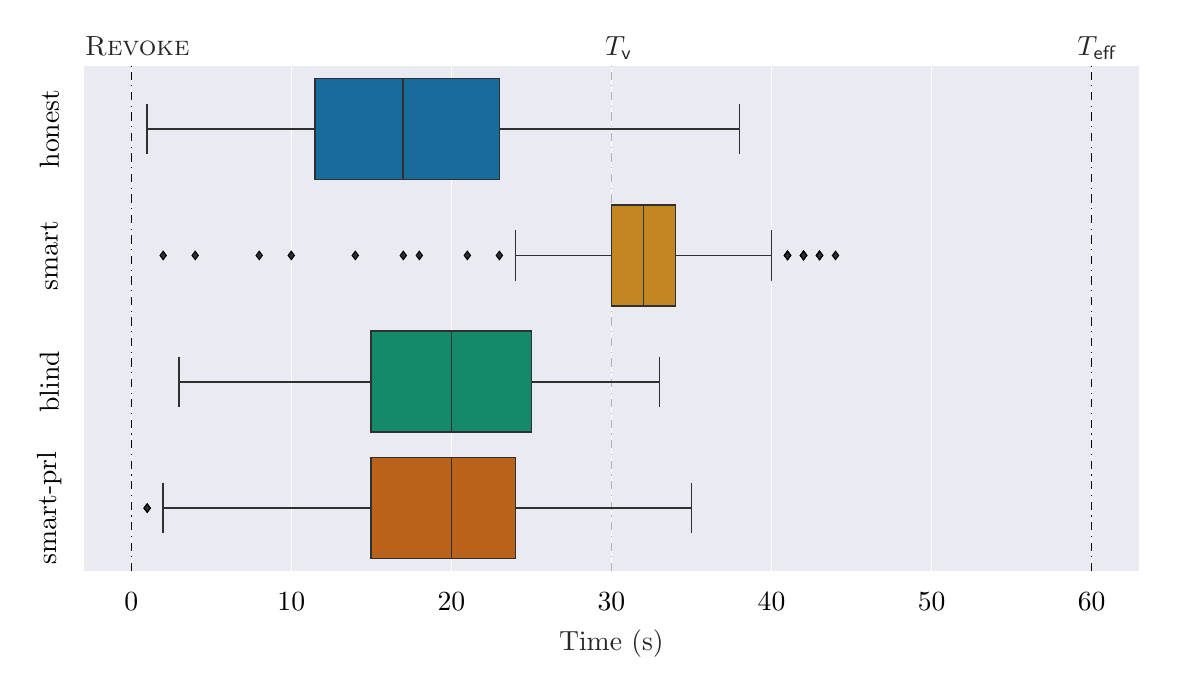
\begin{tikzpicture}

\definecolor{chocolate1869726}{RGB}{186,97,26}
\definecolor{darkgoldenrod19413532}{RGB}{194,135,32}
\definecolor{darkslategray38}{RGB}{38,38,38}
\definecolor{darkslategray48}{RGB}{48,48,48}
\definecolor{lavender234234242}{RGB}{234,234,242}
\definecolor{seagreen21138106}{RGB}{21,138,106}
\definecolor{teal23108155}{RGB}{23,108,155}

\begin{axis}[
clip=false,
axis background/.style={fill=lavender234234242},
axis line style={white},
height=8cm,
minor xtick={},
minor ytick={},
tick align=outside,
width=15cm,
x grid style={white},
xlabel=\textcolor{darkslategray38}{Time (s)},
xmajorgrids,
xmajorticks=true,
xmin=-3, xmax=63,
xtick style={color=darkslategray38,draw=none},
xtick={-10,0,10,20,30,40,50,60,70},
y dir=reverse,
y grid style={white},
ymajorticks=true,
ymin=-0.5, ymax=3.5,
ytick style={color=darkslategray38,draw=none},
ytick={0,1,2,3},
yticklabel style={rotate=90.0,anchor=center,yshift=8pt},
yticklabels={honest,smart,blind,smart-prl}
]
% START VERTICAL LINES %
\addplot [dashdotted, black]
table {%
0 3.5
0 -0.5
};
\addplot [dashdotted, gray!60]
table {%
30 3.5
30 -0.5
};
\addplot [dashdotted, black]
table {%
60 3.5
60 -0.5
};
% END VERTICAL LINES %
\path [draw=darkslategray48, fill=teal23108155, semithick]
(axis cs:11.5,-0.4)
--(axis cs:11.5,0.4)
--(axis cs:23,0.4)
--(axis cs:23,-0.4)
--(axis cs:11.5,-0.4)
--cycle;
\path [draw=darkslategray48, fill=darkgoldenrod19413532, semithick]
(axis cs:30,0.6)
--(axis cs:30,1.4)
--(axis cs:34,1.4)
--(axis cs:34,0.6)
--(axis cs:30,0.6)
--cycle;
\path [draw=darkslategray48, fill=seagreen21138106, semithick]
(axis cs:15,1.6)
--(axis cs:15,2.4)
--(axis cs:25,2.4)
--(axis cs:25,1.6)
--(axis cs:15,1.6)
--cycle;
\path [draw=darkslategray48, fill=chocolate1869726, semithick]
(axis cs:15,2.6)
--(axis cs:15,3.4)
--(axis cs:24,3.4)
--(axis cs:24,2.6)
--(axis cs:15,2.6)
--cycle;
\addplot [semithick, darkslategray48]
table {%
11.5 0
1 0
};
\addplot [semithick, darkslategray48]
table {%
23 0
38 0
};
\addplot [semithick, darkslategray48]
table {%
1 -0.2
1 0.2
};
\addplot [semithick, darkslategray48]
table {%
38 -0.2
38 0.2
};
\addplot [semithick, darkslategray48]
table {%
30 1
24 1
};
\addplot [semithick, darkslategray48]
table {%
34 1
40 1
};
\addplot [semithick, darkslategray48]
table {%
24 0.8
24 1.2
};
\addplot [semithick, darkslategray48]
table {%
40 0.8
40 1.2
};
\addplot [black, mark=diamond*, mark size=1.5, mark options={solid,fill=darkslategray48}, only marks]
table {%
2 1
23 1
10 1
18 1
14 1
4 1
8 1
17 1
21 1
44 1
43 1
41 1
42 1
41 1
42 1
43 1
41 1
43 1
42 1
42 1
};
\addplot [semithick, darkslategray48]
table {%
15 2
3 2
};
\addplot [semithick, darkslategray48]
table {%
25 2
33 2
};
\addplot [semithick, darkslategray48]
table {%
3 1.8
3 2.2
};
\addplot [semithick, darkslategray48]
table {%
33 1.8
33 2.2
};
\addplot [semithick, darkslategray48]
table {%
15 3
2 3
};
\addplot [semithick, darkslategray48]
table {%
24 3
35 3
};
\addplot [semithick, darkslategray48]
table {%
2 2.8
2 3.2
};
\addplot [semithick, darkslategray48]
table {%
35 2.8
35 3.2
};
\addplot [black, mark=diamond*, mark size=1.5, mark options={solid,fill=darkslategray48}, only marks]
table {%
1 3
1 3
};
\addplot [semithick, darkslategray48]
table {%
17 -0.4
17 0.4
};
\addplot [semithick, darkslategray48]
table {%
32 0.6
32 1.4
};
\addplot [semithick, darkslategray48]
table {%
20 1.6
20 2.4
};
\addplot [semithick, darkslategray48]
table {%
20 2.6
20 3.4
};
\draw (axis cs:-3.5,-0.58) node[
  scale=1,
  anchor=base west,
  text=darkslategray38,
  rotate=0.0
]{\textsc{Revoke}};
\draw[dashed] (axis cs:29,-0.58) node[
  scale=1,
  anchor=base west,
  text=darkslategray38,
  rotate=0.0
]{$T_{\mathsf{v}}$};
\draw (axis cs:58.5,-0.58) node[
  scale=1,
  anchor=base west,
  text=darkslategray38,
  rotate=0.0
]{$T_{\mathsf{eff}}$};
\end{axis}

\end{tikzpicture}

    } \caption{Simulation results for $\paramteff{} = 60 s$. The boxes show, for
    each revoked pseudonym, the time between \funcrevokedaa{} and the last
    \funcverify{} event, aggregating more than \simrevocations{} revocations but
    excluding negative values.}
    \label{fig:eval-sim-base}
\end{figure}

\noindent\textbf{\emph{Results.}}
%
The box plots in \cref{fig:eval-sim-base} illustrate the distribution of
revocation times for each attacker level. An additional box plot labeled
\attackersmartprl{} shows simulation results under a \attackersmart{} attacker,
where \acp{TC} use the \ac{PRL} to perform active revocation, as described in
\cref{section:design-extensions}. Each value represents the time between the
revocation of a pseudonym \ps{} (\funcrevokedaa{} event) and the last \ac{V2V}
message signed with \ps{} that was verified by a non-malicious \ac{TC}
(\funcverify{} event). Such time period represents the \emph{effective
revocation time} for that particular pseudonym
(cf.~\cref{section:system-model}).

It should be noted that we filtered out negative time values from the results:
such values represent a situation where the last \funcverify{} event happened
\emph{before} the \funcrevokedaa{} event, for example because the \ac{TC} owner
of the revoked pseudonym was already in a revoked state due to the revocation of
another of its pseudonyms, or simply because that pseudonym was not used to sign
messages in the time after \funcrevokedaa{}. Either way, these values were not
interesting for our evaluation.%\christoph{maybe skip this paragraph for space?}

\cref{fig:eval-sim-base} shows that pseudonyms belonging to \attackerhonest{}
vehicles are revoked rather quickly. Still, as \ac{V2V} messages have a validity
period of \paramtt{} and receiving vehicles' internal time may lag behind the RA
within \paramtt{}, the effective revocation time varied widely, with a median of
\simhonestmedian{} seconds.

The simulation with the \attackersmart{} attacker level resulted in a median of
\simsmartmedian{} seconds and the majority of revocations between \simsmartmin{}
and \simsmartmax{} seconds. %As explained earlier, 
This attacker is able to
postpone revocation by dropping \acp{HB}, yet %but on the other side
not relaying
fresh \acp{HB} eventually causes de-synchronization in the \ac{TC}. Therefore,
in 99\% of cases revocation was effective within 2/3 of \paramteff{},
as honest vehicles were able to stay synchronized with the infrastructure
even when simulating severe network malfunctions.

As for the \attackerblind{} attacker level, we experienced a higher number of
negative values in our results. This can be explained by the fact that a
\attackerblind{} \ac{OBU} is not able to recognize which \acp{HB} can be dropped
or delayed, which ones are fresh and which are old, and which ones can be
delivered to the \ac{TC} without causing revocation. As a result, and
considering the network malfunctions we simulated, the \ac{TC} is more likely to
get de-synchronized and thus automatically revoked, even before revocation is
mandated by the \ac{RA}. This suggests that encrypting \acp{HB} makes it more
difficult for an attacker to evade revocation. In the few cases where the
vehicle was still operating after the \funcrevokedaa{} event, instead,
revocation rarely took longer than \paramtt{}.%\christoph{if we remove the other paragraph we need to explain here that negative values are omitted}

Finally, the \attackersmartprl{} simulation showed a significant improvement
over the \attackersmart{} one, with values more evenly distributed between
\simsmartprlmin{} and \simsmartprlmax{} seconds and median of
\simsmartprlmedian{} seconds. However, these results were negatively affected by
our simulated network malfunctions. As with traditional \acp{CRL}, the ability
of a \ac{TC} to discard messages coming from revoked vehicles depends on how
quickly \acp{HB} are received and processed; Thus, with limited connectivity the
effective revocation time increases. Indeed, we experienced better results when
simulating scenarios with lower drop/delay rates for \acp{HB}.

Overall, our simulations showed the feasibility of our revocation scheme in a
simulated though practical scenario. In the average case, revocation takes much
less than \paramteff{} to be effective, even when attackers attempt to evade it.
Furthermore, simulating network malfunctions did not incur permanent
de-synchronization of non-malicious vehicles, demonstrating the resiliency
of our approach under real-world conditions.
 
\subsection{Size of PRL}
\label{section:eval-prl-size}

The size of a heartbeat is not constant.  Instead, it depends on the size of the
\ac{PRL}, which varies over time according to the number of pseudonyms revoked
and the parameter $T_{prl}$ (\cref{eq:t-prl}). If many pseudonyms are revoked at
the same time, the \ac{PRL} will be large until $T_{prl}$ time has passed and
they are evicted from the \ac{PRL} again. To calculate the expected average
\ac{PRL} size, we approximate adding and removing pseudonyms from the list as a
stochastic process and create a Markov model based on these parameters. The
stationary distribution of this Markov chain then gives the probabilities for
each given size of the \ac{PRL} after an arbitrary number of steps.

Below, we elaborate on the core formulas and the expected values of the \ac{PRL}
size for a chosen set of parameters. Appendix~\ref{appendix:markov} contains a
complete explanation of the utilized probabilities, the Markov model, and a
discussion of the nuances of modelling the \ac{PRL} size as a probabilistic
process.

\noindent\textbf{\emph{PRL as a Markov Model.}}
%
The process of adding and removing pseudonyms from the \ac{PRL} can be seen as a
finite state machine where the states are the possible sizes of the list.
Transitions to a higher or lower state then happen on the addition or removal of
a pseudonym, w.r.t.~a base revocation probability $p$ per pseudonym and time step.  
%In this mental model, the next step in the state
%machine only depends on the current state as well as the parameters describing a
%possible state transition and is independent of the history of the state machine
%before the currently observed state.  
A discrete time Markov chain describes the probability of moving
from state $i$ to state $j$ for each possible state~\cite{hermanns2002markov}.
%The key insight of modelling the PRL as such, if seen as a sequence of probabilistic
%events, we can see the PRL as a Markov model that combines probabilities for
%gaining and losing pseudonyms from the list.
As such, this Markov model represents the probabilities for gaining and losing
pseudonyms from the PRL due to revocation or the removal of pseudonyms after
$\paramtprl{}$, respectively.
%
%\todo[inline]{What are these events, revocation events?}
%
Assuming that the PRL contains $i$ out of $n$ possible pseudonyms at a time
step, we can independently model the probabilities of gaining and losing $k$
pseudonyms as two distinct binomial probabilities $G_{i,k}$ and $L_{i,k}$,
respectively: % as follows:
\begin{equation}
    \label{eq:prl-size-g}
    G_{i,k} = \binom{n-i}{k} \cdot p^k \cdot (1-p)^{n-i-k}  
\end{equation}
\begin{equation}
    \label{eq:prl-size-l}
    L_{i,k} = \binom{i}{k} \cdot (\frac{1}{\paramtprl{}})^{k} \cdot (1-\frac{1}{\paramtprl{}})^{i-k} 
\end{equation}
Observe that $G_{i,k}=0$ if $i+k>n$ and $L_{i,k}=0$ if $i<k$.  We can then
combine these binomial probabilities into a Markov matrix with the following
property:
\begin{align}
    \label{eq:prl-size-markov}
    p_{i,j} = \sum_{l=Max(i-j, 0)}^{i} L_{i,l} \cdot G_{i,l-i+j}
\end{align}

At its core, this Markov matrix contains all probabilities of moving from list
size $i$ to list size $j$ as a combination of losing $l\leq i$ pseudonyms from
the list and adding $l-i+j\leq j$ new ones,   
%Technically, this models the non-deterministic process 
%of removing pseudonyms after $T_{prl}$ time steps as a
%probabilistic process 
where in each time step, a pseudonym is removed from the list with probability
$\frac{1}{\paramtprl{}}$ and added with probability $p$.  While this is not
reasonable to calculate the effective list size after a specific number of
steps, it suffices in a probabilistic model to determine the expected, average
list size.

\noindent\textbf{\emph{Average size of the PRL.}}
%
In Markov chains, a stationary distribution is a state probability that
maintains its distribution even after taking a step in the Markov
chain~\cite{hermanns2002markov}, represented by the stationary vector of the
Markov matrix. It is thus a probabilistic equilibrium that, once reached, will
be stable forever.  After startup, a Markov chain will eventually reach its
stationary distribution after enough steps have been taken.  We can calculate
the equilibrium for our Markov chain for parameters that are useful in the real
world and for different revocation probabilities. By accumulating the
probabilities for each given state, we can thus calculate the maximum list size
as a percentile of possible states.

We evaluate the impact of a growing share of attackers on the PRL size in
the context of two baseline scenarios. In these scenarios,
\textit{honest} pseudonyms, i.e., pseudonyms in the network that do not belong
to attackers, may still experience a seldom revocation due to erroneous
behavior, e.g., due to a faulty sensor. In the first baseline scenario, we
consider a $1\%$ probability that a pseudonym gets revoked at least once within
a day, i.e., a $1\%$ chance for an expected revocation every 86400 time steps of
one second each. In the second scenario, we raise this to the extreme case of a
$99\%$ probability of being revoked at least once a day or 86400 time steps.

\Cref{fig:eval-prl-size} depicts the 75th, 90th, and 99.99th percentiles of the
\ac{PRL} sizes for these two scenarios.  The plot uses the parameters of $n=800$
pseudonyms and $\paramtprl{}=30$, to align with the evaluation described in
\cref{section:eval-sim}.  Each honest lifetime scenario is paired with a growing
share of attackers in the network. Attackers are modeled to
have a $75\%$ chance of causing a pseudonym revocation every 30 minutes on
average, which simulates a strain on the \ac{PRL} that is by magnitudes larger
than any honest pseudonym would normally incur.

In most situations, the \ac{PRL} contains fewer than 10 and 12
pseudonyms for the two baseline scenarios, respectively. Even
with a share of 20\% of network participants that cause revocations heavily, the
99.99th percentile of \ac{PRL} size still stays below 17. This means that
even for coordinated peak revocation events, the \ac{PRL} size
will stay in very manageable margins. For comparison, we estimated the expected
number of revocations over a day: they range from roughly 8 to 10500 for Scenario
1, and 3600 to 13500 for Scenario 2 -- a worst case average of one revocation
every 6-8s.

% \begin{figure*}[ht]
%     \centering
%     \begin{subfigure}{.5\textwidth}
%       \centering
%       \includegraphics[width=.8\linewidth]{figures/60.png}
%       \caption{$T_{prl} = 60s$}
%     \end{subfigure}%
%     \begin{subfigure}{.5\textwidth}
%       \centering
%       \includegraphics[width=.8\linewidth]{figures/300.png}
%       \caption{$T_{prl} = 300s$}
%     \end{subfigure}
%     \caption{Results of our simulation on the evolution of the \ac{PRL} size
%     over time, each second revoking a pseudonym non-deterministically with
%     probability 0.1. After an initial growth, the number of elements in the list
%     fluctuates around $T_{prl} * 0.1$.}
%     \label{fig:eval-prl-size}
% \end{figure*}


% Adjustments to auto generated plot:
% 1 to axis add 
% width=\columnwidth,
% legend pos=north west,
% xticklabel style = {
%       /pgf/number format/fixed,
%       /pgf/number format/precision=6
%   },
% scaled x ticks=false,
% T_PRL = 300
% n=400
% 

\begin{figure}[t]
\centering
% This file was created with tikzplotlib v0.10.1.
% This file was created with tikzplotlib v0.10.1.
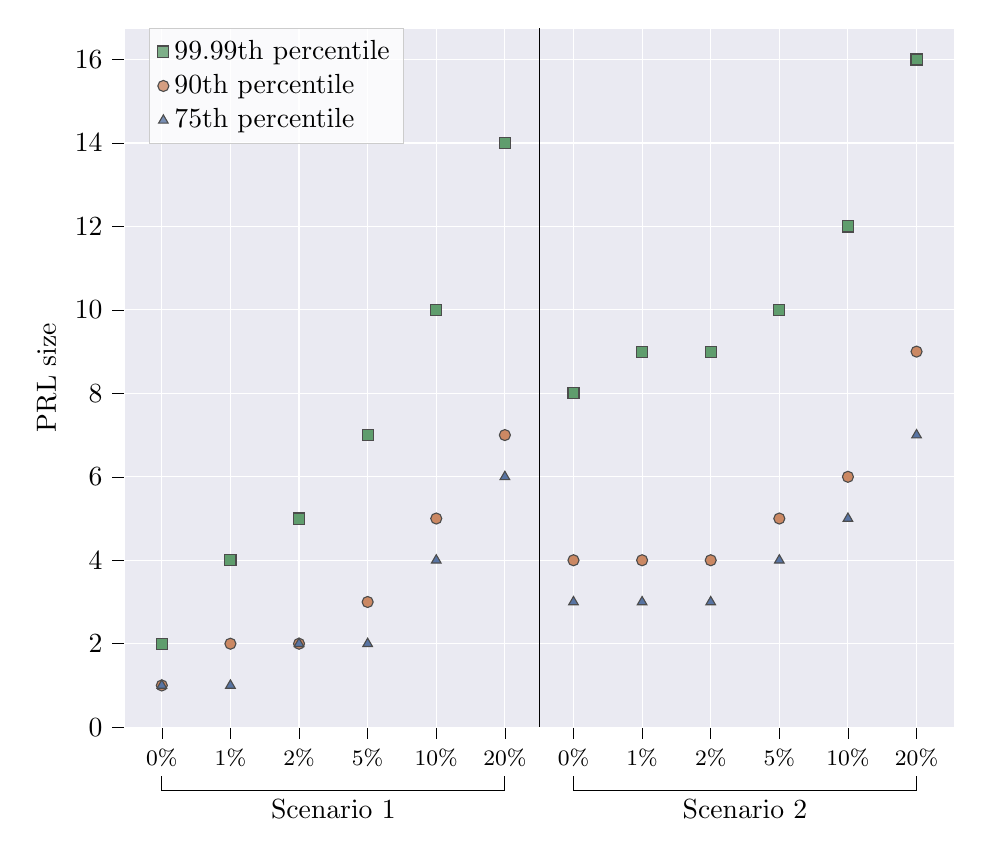
\begin{tikzpicture}

  \definecolor{lightgray204}{RGB}{204,204,204}
  \definecolor{darkslategray38}{RGB}{38,38,38}
  \definecolor{darkslategray76}{RGB}{76,76,76}
  \definecolor{indianred1819295}{RGB}{181,92,95}
  \definecolor{lavender234234242}{RGB}{234,234,242}
  \definecolor{lightslategray133122170}{RGB}{133,122,170}
  \definecolor{mediumseagreen95157109}{RGB}{95,157,109}
  \definecolor{peru20313699}{RGB}{203,136,99}
  \definecolor{steelblue76114176}{RGB}{76,114,176}
  \definecolor{steelblue88116163}{RGB}{88,116,163}
  
  \begin{axis}[
    width=\columnwidth,
    ylabel= PRL size,
    xmajorgrids,
    xmajorticks=true,
    ymajorgrids,
    ymajorticks=true,
    axis background/.style={fill=lavender234234242},
    axis line style={white},
    x grid style={white},
    y grid style={white},
  legend cell align={left},
  legend style={
    fill opacity=0.8,
    draw opacity=1,
    text opacity=1,
    at={(0.03,1.0)},
    anchor=north west,
    draw=lightgray204
  },
  tick align=outside,
  tick pos=left,
  % x grid style={darkgray176},
  xmin=-0.55, xmax=11.55,
  xtick style={color=black},
  xtick={0,1,2,3,4,5,6,7,8,9,10,11},
  xticklabel style={name=tick no \ticknum, font=\footnotesize},
  xticklabels={
    $0\%$,
    $1\%$,
    $2\%$,
    $5\%$,
    $10\%$,
    $20\%$,
    $0\%$,
    $1\%$,
    $2\%$,
    $5\%$,
    $10\%$,
    $20\%$
  },
  % y grid style={darkgray176},
  ymin=0.0, ymax=16.75,
  ytick style={color=black}
  ]
  \addplot [draw=darkslategray76, fill=mediumseagreen95157109, mark=square*, only marks]
  table{%
x  y
0 2
1 4
2 5
3 7
4 10
5 14
6 8
7 9
8 9
9 10
10 12
11 16
};
\addlegendentry{99.99th percentile}
\addplot [draw=darkslategray76, fill=peru20313699, mark=*, only marks]
table{%
x  y
0 1
1 2
2 2
3 3
4 5
5 7
6 4
7 4
8 4
9 5
10 6
11 9
};
\addlegendentry{90th percentile}
\addplot [draw=darkslategray76, fill=steelblue88116163, mark=triangle*, only marks]
table{%
x  y
0 1
1 1
2 2
3 2
4 4
5 6
6 3
7 3
8 3
9 4
10 5
11 7
};
\addlegendentry{75th percentile}

\draw (axis cs:5.5,0) -- (axis cs:5.5,45);

% \draw (axis cs:0.0, -2) -- (axis cs:0.0, -4) -- (axis cs:5.0, -4) -- (axis cs:5.0, -2);


\end{axis}
\draw  (tick no 0.south) -- +(0,-.5em) -- ([yshift=-.5em] tick no 5.south)  node [midway, below] {Scenario 1}  -- +(0,.5em);
\draw  (tick no 6.south) -- +(0,-.5em) -- ([yshift=-.5em] tick no 11.south) node [midway, below] {Scenario 2} -- +(0,.5em);
  
  \end{tikzpicture}
  
\caption{Markov model percentiles for maximum PRL sizes for $T_{prl}=30s$,
  $n=800$, and different shares of attackers in each baseline revocation
  scenario.}
\label{fig:eval-prl-size}
\end{figure}


\subsection{Choice of \paramtt{}}
\label{section:eval-tv}

\begin{figure}[t]
  %\centering
  \hspace*{-0.3cm}
  \resizebox{\linewidth}{!} {
    % This file was created with tikzplotlib v0.10.1.
\begin{tikzpicture}

\definecolor{chocolate213940}{RGB}{213,94,0}
\definecolor{darkcyan1115178}{RGB}{1,115,178}
\definecolor{darkcyan2158115}{RGB}{2,158,115}
\definecolor{darkgray176}{RGB}{176,176,176}
\definecolor{darkorange2221435}{RGB}{222,143,5}

\begin{groupplot}[group style={vertical sep=3.5cm, horizontal sep=2.5cm,group size=2 by 2}]
\nextgroupplot[
height=6cm,
minor xtick={},
minor ytick={},
tick align=outside,
tick pos=left,
title={\(\displaystyle T_{eff}\) (min)},
width=15cm,
x grid style={darkgray176},
xmin=-13.5, xmax=943.5,
xtick style={color=black,draw=none},
xtick={30,150,300,900},
y grid style={darkgray176},
ymin=-0.45, ymax=31.45,
ytick style={color=black,draw=none},
ytick={-10,0,10,20,30,40},
clip=false,
label style={font=\Huge},
tick label style={font=\Huge},
title style={font=\Huge}
]
\addplot [semithick, darkcyan1115178]
table {%
30 1
150 5
300 10
900 30
};

\nextgroupplot[
height=6cm,
minor xtick={},
minor ytick={},
tick align=outside,
tick pos=left,
title={HB frequency (HB/min)},
width=15cm,
x grid style={darkgray176},
xmin=-13.5, xmax=943.5,
xtick style={color=black,draw=none},
xtick={30,150,300,900},
y grid style={darkgray176},
ymin=-0.9, ymax=62.9,
ytick style={color=black,draw=none},
ytick={-20,0,20,40,60,80},
clip=false,
label style={font=\Huge},
tick label style={font=\Huge},
title style={font=\Huge}
]
\addplot [semithick, darkorange2221435]
table {%
30 60
150 12
300 6
900 2
};

\nextgroupplot[
height=6cm,
minor xtick={},
minor ytick={},
tick align=outside,
tick pos=left,
title={HB size (KB)},
width=15cm,
x grid style={darkgray176},
xmin=-13.5, xmax=943.5,
xtick style={color=black,draw=none},
xtick={30,150,300,900},
y grid style={darkgray176},
ymin=1.0832, ymax=11.2208,
ytick style={color=black,draw=none},
ytick={0,5,10,15},
clip=false,
label style={font=\Huge},
tick label style={font=\Huge},
title style={font=\Huge}
]
\addplot [semithick, darkcyan2158115]
table {%
30 1.544
150 3.272
300 5.064
900 10.76
};

\nextgroupplot[
height=6cm,
minor xtick={},
minor ytick={},
tick align=outside,
tick pos=left,
title={Required bandwidth (KBit/s)},
width=15cm,
x grid style={darkgray176},
xmin=-13.5, xmax=943.5,
xtick style={color=black,draw=none},
xtick={30,150,300,900},
y grid style={darkgray176},
ymin=2.3952, ymax=12.8261333333333,
ytick style={color=black,draw=none},
ytick={0,5,10,15},
clip=false,
label style={font=\Huge},
tick label style={font=\Huge},
title style={font=\Huge}
]
\addplot [semithick, chocolate213940]
table {%
30 12.352
150 5.2352
300 4.0512
900 2.86933333333333
};
\end{groupplot}

\end{tikzpicture}

  } \caption{Evaluation of the impact of \paramtt{} on the \ac{V2X} system. The
  X axes show the value of \paramtt{} in seconds.}
  \label{fig:eval-tv}
\end{figure}

The choice of \paramtt{} is crucial in our scheme. We evaluated four reference
values of 30, 150, 300 and 900 seconds and visualize the results in
\cref{fig:eval-tv}. Below, we discuss the impact of \paramtt{} across multiple
dimensions. 

\noindent\textbf{\emph{Revocation time.}}
%
The first dimension is related to the revocation time, and is shown in the
top-left plot of \cref{fig:eval-tv}. According to
\cref{eq:effective-revocation}, the effective revocation time \paramteff{} is
linearly dependent on \paramtt{}. Therefore, the smaller \paramtt, the shorter
it takes to revoke, resulting in a safer system.

\noindent\textbf{\emph{\ac{HB} frequency.}}
%
The frequency with which \acp{HB} are generated and distributed by the \ac{RA}
is not fixed arbitrarily, but depends on \paramtt{}. Here, it is essential to
ensure that honest vehicles remain loosely synchronized with the infrastructure
during their operation. This means that, to avoid temporary service
interruption, \acp{TC} need to process \emph{at least} one \ac{HB} every
\paramtt{} (cf.~\cref{chapter:design}). Thus, the frequency of \acp{HB} is
inversely proportional to the value of \paramtt{} with a certain coefficient
$N$, which accounts for network latencies and missing packets. The top-right
plot of \cref{fig:eval-tv} shows the frequency with coefficient $N = 30$, i.e.,
a new \ac{HB} is generated every $\paramtt / 30$ seconds. With larger
\paramtt{}, the number of \acp{HB} per minute drastically decreases, resulting
in fewer resources used.

\noindent\textbf{\emph{\ac{HB} size.}}
%
According to \cref{eq:heartbeat-format}, the size of a \ac{HB} is linearly
dependent on the size of the \ac{PRL}, plus a constant value that represents the
sizes of timestamp \paramthb{} and digital signature \funcsignature{}.
Additionally, as discussed in \cref{section:eval-prl-size}, the size of the
\ac{PRL} is directly impacted by the value of \paramtt{}. That is, the higher
\paramtt{} is chosen, the longer each pseudonym needs to stay in the \ac{PRL},
according to \cref{eq:t-prl}. This means that, on average, \acp{HB} are bigger
when \paramtt{} increases. The bottom-left plot of \cref{fig:eval-tv} shows the
\ac{HB} size when varying \paramtt{}, considering the 99.99 percentile of the
\ac{PRL} size in relation to \paramtt{} on the worst case scenario, i.e.,
Scenario 2 with 800 pseudonyms and 20\% of attackers in the network
(cf.~\cref{fig:eval-prl-size}). We also assume that a pseudonym identifier is 64
bytes, \paramthb{} is 8 bytes, and we overestimate the size of \funcsignature{}
to 512 bytes, which is higher than most RSA and elliptic curve
signatures~\cite{nistDSS}.

\noindent\textbf{\emph{Network bandwidth.}}
%
Lastly, it is important to evaluate the network bandwidth required for
transmitting \acp{HB}. This can be computed by multiplying the size of a \ac{HB}
by the frequency with which \acp{HB} are distributed. Results show that the
minimum bandwidth needed to transmit \acp{HB} is rather small, i.e., around 12
KBit/s in the worst-case scenario and with large $N$.

\noindent\textbf{\emph{Conclusions.}}
%
The choice of \paramtt{} should be a good compromise between security and
usability. The smaller \paramtt{} is, the shorter a revocation takes, but it
also increases the resources used and the risk of de-synchronization in honest
vehicles. Besides, a small \paramtt{} is feasible when the \ac{V2X} network is
reliable and low-latency, e.g., in urban areas, but may not be always practical,
e.g., in rural areas. On the other hand, a large \paramtt{} results in a more
resilient and efficient \ac{V2X} system at the cost of a slower revocation.
However, compared with passive revocation
(cf.~\cref{section:discussion-comparison}), even \paramteff{} values of 30
minutes are a significant improvement on the revocation time, coming at
negligible cost, as shown in \cref{fig:eval-tv}.
